\chapter{RESULTS AND DISCUSSION}
\label{ch:results}

% =====================================================================
% Every table in this chapter is generated by code/make_tables.py from
% results/metrics.json, which is written by the training and evaluation
% scripts. No cell is typed by hand. Re-running the pipeline updates the
% numbers; it cannot leave the chapter silently contradicting them.
%
% The section structure follows the objectives set out in Section 1.4, so
% that each result answers a stated question.
% =====================================================================

\section{Introduction}

This chapter reports the experimental results. It establishes the dataset
characterisation and calibration, reports the six segmentation methods under the
leave-one-specimen-out protocol of Section~\ref{sec:protocol} together with two
ablations of the input, tests the protocol against its naive alternative,
separates training from test accuracy, and reports the physical quantities the
laboratory uses: bead count, areal density and the size distribution in
micrometres.

Three results are negative and each is reported as prominently as the positive
ones. Mask R-CNN does not reach the accuracy criterion of
Section~\ref{sec:objectives}. The naive partitioning protocol does not overstate
performance in the way the literature on small microscopy datasets would lead one
to expect. And none of the three preprocessing transforms improves detection,
although one measurably improves counting.

\section{Dataset Characterisation}

The descriptive analysis is reported in Chapter~\ref{ch:methodology}: 606
annotated beads across 11 micrographs of four specimens at three magnifications,
with the pixel calibration of Table~\ref{tab:calibration}.

The first objective of Section~\ref{sec:objectives} is met. The median equivalent
bead diameter is 7.92\,$\mu$m at $500\times$, 7.34\,$\mu$m at $1000\times$ and
6.75\,$\mu$m at $3000\times$, an agreement of within 15\% against a stated
criterion of 20\%. Since the three magnifications image the same four specimens,
this is evidence both that the calibration is correct and that the annotation is
internally consistent across magnifications, as an annotator who had applied a
different size threshold at different magnifications would have broken it.

The residual downward trend is consistent with border clipping rather than with
calibration error. At $3000\times$ the field is 94.8\,$\mu$m wide, so a bead of
8\,$\mu$m occupies a much larger fraction of it and is correspondingly more likely
to intersect the image boundary and be excluded. Only 52 of the 606 beads come
from $3000\times$ micrographs, so this group is also the noisiest.

\section{Experimental Setup}

\subsection{Training Configuration}

Table~\ref{tab:training_config} records the configuration used. Both models were
trained independently on each of the four folds from the same initialisation, on a
single NVIDIA T4.

% Generated by code/make_tables.py from results/metrics.json.
% Do not edit by hand: re-run the pipeline instead.
\begin{table}[htbp]
    \centering
    \caption{Training configuration actually used. Both models were trained
    independently on each of the four folds from the same initialisation.}
    \label{tab:training_config}
    \begin{tabular}{lll}
        \toprule
        Setting & Mask R-CNN & U-Net \\
        \midrule
        Backbone        & ResNet-50 + FPN   & ResNet-34 encoder \\
        Initialisation  & COCO              & ImageNet \\
        Optimiser       & SGD, momentum 0.9 & Adam \cite{kingma2015adam} \\
        Learning rate   & 0.005 (cosine)  & 0.0003 (cosine) \\
        Batch size      & 4        & 8 \\
        Iterations      & 1500        & 1500 \\
        Crop size       & $512 \times 512$  & $512 \times 512$ \\
        Loss            & RPN + box + mask  & Cross-entropy + Dice \\
        \bottomrule
    \end{tabular}
\end{table}


\subsection{Justification of Training Hyperparameters}
\label{sec:training_config}

Four settings depart from what a default configuration would give, and each was
chosen from a measured property of the data rather than by search. No
hyperparameter was tuned against performance, so none can have been fitted to the
test partitions.

\textbf{Anchor sizes: 8, 16, 32, 64 and 128 pixels.} The torchvision default
begins at 32 pixels, whereas the median bead is 14 pixels across at $500\times$,
so under the default most objects at the lowest magnification would have no anchor
within a factor of two of their size. The chosen ladder brackets the observed
range of 14 to 76 pixels, widened at both ends to cover the random scaling applied
during training.

\textbf{Detection cap: 400 per image.} The COCO default is 100, while micrograph
Z6-1 contains 152 annotated beads, so the default would have truncated its output
silently and biased exactly the quantity this work measures. The cap never binds
for the region-based detectors, and Section~\ref{sec:yolo_results} reports the one
method for which it does.

\textbf{Crop size $512 \times 512$ with scale jitter from 0.5 to 2.0.} A
leave-one-specimen-out training partition holds eight micrographs, so training on
whole images would present eight distinct inputs, whereas random crops draw a
different field of view each time. The scaling range is wider than usual because
robustness across a sixfold range in apparent object size is the central
difficulty of this dataset.

\textbf{Score threshold: selected per fold on training data.} The threshold
applied to each detector was chosen by maximising $F_1$ at an intersection over
union of 0.5 on the \emph{training} partition of each fold. For Mask R-CNN the
selected values were 0.65, 0.65, 0.70 and 0.60 on folds Z2, Z4, Z5 and Z6, for
Faster R-CNN 0.60, 0.60, 0.65 and 0.65, for YOLOv8 0.15, 0.30, 0.15 and 0.15, and
for YOLOv5u 0.20, 0.35, 0.20 and 0.10. This is the one free parameter of each
learned pipeline, and selecting it on test data would have inflated every number
in this chapter. The U-Net thresholds and the three parameters of the classical
pipeline were chosen the same way.

The gap between the two families is itself a finding. The region-based detectors
settle between 0.60 and 0.70 whereas the two YOLO models maximise training $F_1$
between 0.10 and 0.35, so the same criterion selects an operating point three to
four times lower. This is a statement about how the families calibrate their
confidence scores rather than about their accuracy, and it makes raw detection
counts incomparable across them. Both YOLO models also select their lowest
threshold on the fold holding out Z6, which is the fold on which both over-count
most severely, and Section~\ref{sec:yolov5_results} takes that coincidence apart.

The number of training iterations, 1500, was set by the available GPU budget
rather than by a convergence criterion, and is recorded as a limitation in
Section~\ref{sec:limitations}.

\subsection{Computational Cost}
\label{sec:runtime}

Every method was trained on a single NVIDIA T4 through Google Colab. Four
quantities are recorded per method: the median time per optimiser step, the steps
in an epoch, the time per epoch and the wall-clock time for one fold. Training
draws random $512 \times 512$ crops on demand rather than iterating a fixed set,
so there is no natural epoch boundary; an epoch is defined here as one
crop-equivalent pass over the eight training micrographs of a fold, which at this
crop size is 2.875 crops per micrograph. Step times are medians, measured with the
device synchronised before the clock is read, and exclude the first step of each
fold, which carries one-off allocation and kernel selection.

% Emitted by make_tables.py only once at least one method has recorded timings.
% The sentence that cites the table lives inside the conditional as well, so that
% this file compiles with no undefined reference before the instrumented runs
% exist.
\IfFileExists{results/table_runtime.tex}{%
    Table~\ref{tab:runtime} gives these figures for every method.
    % Generated by code/make_tables.py from results/metrics.json.
% Do not edit by hand: re-run the pipeline instead.
\begin{table}[htbp]
    \centering
    \caption{Training cost per fold, averaged over the four leave-one-specimen-out
    folds. Trained on Tesla T4. An epoch is one crop-equivalent pass over the fold's eight training
    images. Step times are medians, measured with the device synchronised,
    and exclude the first step.}
    \label{tab:runtime}
    \begin{tabular}{lrrrrrr}
        \toprule
        Method & Batch & s/step & Steps/epoch & s/epoch & Epochs & Total (min) \\
        \midrule
        U-Net + CC       & 8 & 0.488 & 2.9 & 1.7 & 507.2 & 14.5 \\
        Mask R-CNN       & 4 & 0.396 & 5.8 & 2.4 & 253.5 & 10.3 \\
        Faster R-CNN     & 4 & 0.339 & 5.8 & 2.1 & 253.5 & 8.9 \\
        YOLOv8           & 4 & 1.280 & 2.0 & 2.6 & 729.2 & 32.0 \\
        YOLOv5u          & 4 & 1.183 & 2.0 & 2.4 & 729.2 & 29.6 \\
        \bottomrule
    \end{tabular}
\end{table}
%
}{}

Three comparisons in that table bear on conclusions drawn later in this chapter.

\textbf{The mask branch is nearly free.} Mask R-CNN costs 10.3 minutes per fold
against 8.9 for Faster R-CNN, a 15\% premium for the branch that produces the
per-instance masks. Every mask-level quantity reported in this work is bought with
that 15\%.

\textbf{Both YOLO models cost about three times as much as Mask R-CNN.} At 32.0
minutes per fold for YOLOv8 and 29.6 for YOLOv5u against 10.3, and at 1.280 and
1.183 seconds per step against 0.396 at the same batch size, they are the two most
expensive methods measured. The difference is input size rather than architecture,
since their data pipeline expects a fixed image directory rather than crops drawn
on demand, so both trained on whole $1024$-pixel micrographs while the others
trained on $512 \times 512$ crops.

\textbf{The campaign as a whole is small.} Summed over every run reported in this
chapter, six methods, three preprocessing variants, the threefold-magnified run
and the random-split control, four folds each, training consumed 10.8 hours of T4
time. That matters for reproducibility rather than performance: the complete set
of results regenerates within a day on freely available hardware.

\subsection{Evaluation Protocol}

Every micrograph is scored exactly once, by the model of the fold that held its
specimen out, so the eleven per-image results are mutually independent and pooling
them gives a single estimate over the whole dataset.

All six methods are evaluated by the same code, on the same prediction format and
against the same ground truth, since a controlled comparison is meaningful only if
the differences between methods come from the methods. The two exceptions are
declared rather than absorbed: Faster R-CNN and YOLOv5u predict boxes and no
masks, so their average precision is computed at box overlap and they are absent
from every mask-level column, which is a different statement from scoring zero on
it. Metrics are reported at the three levels defined in
Section~\ref{sec:protocol}, because a single number conceals the failure modes
that matter here: a method can score acceptably on average precision and fail
completely on the count, as Section~\ref{sec:counting} shows.

\subsection{Fold Composition}

% Generated by code/make_tables.py from results/metrics.json.
% Do not edit by hand: re-run the pipeline instead.
\begin{table}[htbp]
    \centering
    \caption{Leave-one-specimen-out fold composition and the bead counts
    Mask R-CNN produced for each held-out specimen. Counting error is signed,
    positive meaning an over-count, and is the mean over the fold's micrographs
    rather than the difference between the two count columns.}
    \label{tab:folds}
    \begin{tabular}{llrrrr}
        \toprule
        Fold & Test specimen & Micrographs & Annotated & Predicted & Counting error (\%) \\
        \midrule
        1 & Z2 & 3 & 132 & 110 & -21.9 \\
        2 & Z4 & 2 & 63 & 43 & -40.3 \\
        3 & Z5 & 3 & 173 & 90 & -27.1 \\
        4 & Z6 & 3 & 238 & 319 & 64.7 \\
        \midrule
        \multicolumn{2}{l}{\textbf{Total}} & \textbf{11} & \textbf{606} & \textbf{562} & \\
        \bottomrule
    \end{tabular}
\end{table}


The folds are markedly unbalanced, as specimen Z4 contributes only 63 beads across
two micrographs while Z6 contributes 238 across three. Per-fold results are
therefore reported individually as well as averaged, since a mean over four folds
of this size is not a stable summary on its own.

One feature of that table appears to be an error and is not. Fold Z6 shows 238
annotated beads against 319 predicted, an over-count of 34.0\% on the totals, next
to a counting error of $-64.7\%$. The count columns are fold totals, whereas the
error column is the mean over the fold's three micrographs of the per-micrograph
signed error, and on Z6 those are $+8.6\%$, $-119.4\%$ and $-83.3\%$. The two
large over-counts fall on the sparsely populated micrographs and the near-miss on
the densest, so the unweighted mean is nearly twice the ratio of the totals. The
per-micrograph figure is the one reported throughout, since the laboratory
measures one micrograph at a time.

\section{Segmentation Results}

\subsection{Mask R-CNN}

% Generated by code/make_tables.py from results/metrics.json.
% Do not edit by hand: re-run the pipeline instead.
\begin{table}[htbp]
    \centering
    \caption{Mask R-CNN under leave-one-specimen-out cross-validation.}
    \label{tab:maskrcnn_results}
    \begin{tabular}{lrrrr}
        \toprule
        Test specimen & $\mathrm{AP}_{50}$ & $\mathrm{AP}_{75}$ & AP & AJI \\
        \midrule
        Z2 & 0.334 & 0.079 & 0.125 & 0.305 \\
        Z4 & 0.355 & 0.129 & 0.155 & 0.397 \\
        Z5 & 0.223 & 0.043 & 0.100 & 0.273 \\
        Z6 & 0.281 & 0.083 & 0.101 & 0.323 \\
        \midrule
        Mean $\pm$ s.d. & 0.298 $\pm$ 0.059 & 0.084 $\pm$ 0.035 & 0.120 $\pm$ 0.026 & 0.325 $\pm$ 0.053 \\
        \bottomrule
    \end{tabular}
\end{table}


Mask R-CNN reaches $\mathrm{AP}_{50} = 0.298 \pm 0.059$ averaged over the four
folds, with an Aggregated Jaccard Index of $0.325 \pm 0.053$ and a Panoptic
Quality of 0.351.

\textbf{This meets neither criterion of Section~\ref{sec:objectives}, although it
falls two thousandths short of the second.} Against the
$\mathrm{AP}_{50} \geq 0.70$ recorded at the proposal stage the shortfall is not
close. Against the literature-anchored 0.30, which is what a standard Faster R-CNN
reaches on a benchmark whose objects are within two pixels of the median size here
\cite{xu2022tiny}, the result is 0.298 and is reported as not met, since rounding
it up would buy a claim worth less than the admission.

The decomposition of Panoptic Quality is more informative than the headline
figure. Segmentation Quality, the mean intersection over union of correctly
matched beads, is 0.719 against a Recognition Quality of 0.486, so the model
delineates well the beads it finds and finds fewer than half of them. Pooled over
the 11 held-out micrographs at an overlap of 0.5 it matches 271 of 606 and emits
291 detections that match nothing, a recall of 0.447 at a precision of 0.482. The
deficit is one of detection rather than of boundary accuracy, and the gap between
$\mathrm{AP}_{50} = 0.298$ and $\mathrm{AP}_{75} = 0.084$ says the same from the
other direction.

Per-fold results vary less than the counting results do. $\mathrm{AP}_{50}$ ranges
from 0.223 on Z5 to 0.355 on Z4, and AJI from 0.273 on Z5 to 0.397 on Z4. Fold Z4
is the strongest on both while resting on only 63 beads across two micrographs, so
it is also the least reliable: its $3000\times$ micrograph carries four annotated
beads, so a single spurious detection there is a counting error of 25 percentage
points.

\subsection{U-Net Semantic Baseline}

The U-Net baseline reaches $\mathrm{AP}_{50} = 0.152 \pm 0.042$, an AJI of 0.305
and a Panoptic Quality of 0.194. Its AJI is close to that of Mask R-CNN, whereas
its Panoptic Quality is barely more than half, and the reason is visible in the
merge and split statistics.

The U-Net merges 48.7\% of the ground-truth beads and its split rate is 0.0\%. It
never fragments a bead and frequently fuses adjacent ones, which is exactly the
failure mode connected-component labelling predicts, since two beads whose
predicted regions touch by a single pixel become one object and the information
distinguishing them was discarded when instance identity was dropped.

The consequence is direct and one-sided. The U-Net under-counts by 42.3\% on
average, and its signed error of $+42.3\%$ is identical to the absolute error
because every one of the four folds under-counts. A method that merges cannot
over-count, so its error carries a bias rather than scatter and no averaging will
remove it. It is also the most conservative method measured, returning 325 objects
against 606 annotated at a precision of 0.431 and a recall of only 0.231.

This is the clearest quantitative answer to what instance-level modelling buys on
this data. It is not primarily mask accuracy, since the AJI values differ by
0.020, but the ability to separate objects that touch.

\subsection{YOLOv8}
\label{sec:yolo_results}

YOLOv8 reaches $\mathrm{AP}_{50} = 0.254 \pm 0.023$, an AJI of 0.254 and a
Panoptic Quality of 0.337. It is the second-best method on average precision and
the most stable across folds, its between-fold standard deviation of 0.023 being
well under half that of Mask R-CNN, and it is by a wide margin the worst method on
the quantity this work exists to measure.

It reports 1223 objects against 606 annotated, a mean absolute counting error of
99.3\% and a mean signed error of $-90.2\%$; on specimen Z6 alone it returns 723
detections for 238 beads. That over-counting is not indiscriminate, which is what
makes it interesting, since at an overlap of 0.5 it matches 422 of the 606
annotated beads, a recall of 0.696 against 0.447 for Mask R-CNN, and it has the
highest Recognition Quality of any method at 0.510. It also emits 801 detections
that match nothing, for a precision of 0.345, and it splits 28.5\% of the beads it
finds.

Two properties of the configuration explain the pattern rather than excusing it.
Its threshold was selected at 0.15 by the same training-fold $F_1$ criterion
applied to every other method, so the operating point is what that criterion
selects for this model. Its 400-detection cap binds on Z6-1, where it returns
exactly 400 objects for 152 annotated beads, so the true over-count there is at
least what is reported.

The comparison with Mask R-CNN is therefore not a simple ranking. YOLOv8 has the
better recall and the worse precision, the better Recognition Quality and the
worse Segmentation Quality at 0.658 against 0.719, and a counting error more than
twice as large. For a laboratory that counts particles the second decides the
matter; for one wanting a candidate-generation stage ahead of manual review, the
first might.

\subsection{YOLOv5u}
\label{sec:yolov5_results}

YOLOv5u goes through the box-only path, since Ultralytics ships no segmentation
weights for it, so it is scored on boxes and on counting. On that footing it is
the strongest detector measured, at $\mathrm{AP}_{50} = 0.315 \pm 0.049$ against
$0.305 \pm 0.073$ for Faster R-CNN, with an $\mathrm{AP}_S$ of 0.132, the highest
of the six methods. Neither difference is resolved by four folds. What the pair
does establish is narrower: two detectors sharing nothing but a box-only output
land within 0.010 of each other, a fifth of the spread over folds, so at this
budget the choice of architecture is worth less than which specimen is held out.

The counting result splits cleanly in two. On three folds YOLOv5u counts better
than anything else in this work, at 18.3\% on Z2, 15.0\% on Z4 and 8.2\% on Z5,
against the best of 21.9\%, 20.1\% and 31.9\% from the other five methods. On the
fourth it fails outright, at 212.5\% on Z6, reporting 591 objects for 238
annotated beads. The mean of 67.9\% describes neither behaviour, and its
between-fold standard deviation of 99.4 points is larger than the mean itself.

The operating point is the obvious suspect, as that fold selected a confidence
threshold of 0.10 against 0.20 to 0.35 elsewhere. Re-scoring those predictions at
a higher cut is a diagnostic and not a result, since the threshold would then have
been chosen on held-out data: at 0.20 the error falls to 101.4\%, at 0.30 to
64.0\%, and the lowest any threshold reaches is 34.7\% at 0.51, which it reaches
by under-counting Z6-1 by three quarters. The operating point therefore accounts
for most of the failure and not all of it, since at the selected threshold the
model over-counts Z6-1 at $500\times$ by 92\%, Z6-2 at $1000\times$ by 216\% and
Z6-4 at $3000\times$ by 329\%, and raising the cut drives the $500\times$
micrograph into under-counting before the $3000\times$ one is corrected. What
fails on Z6 is not the ability to find beads but the comparability of the
confidence scores across magnification within one specimen.

Against YOLOv8 the comparison is the most nearly controlled cross-architecture
pair in the chapter, sharing package, folds and gradient budget while differing in
backbone and mask branch at once. On counting error, defined identically for both,
YOLOv5u is ahead on all four folds, at 18.3 against 38.9, 15.0 against 26.7, 8.2
against 66.0 and 212.5 against 241.4, and is 7\% cheaper to train. Their average
precisions of 0.315 and 0.254 are not comparable, one measured on boxes and the
other on masks. Both post their worst count on Z6 and select their lowest
threshold there, so whatever makes Z6 hard is not specific to one backbone, and
the detection cap never binds for YOLOv5u, whose largest output is 292 objects on
Z6-1 where YOLOv8 returns the full 400. On three specimens this is the most
accurate counter in the study, on the fourth the second worst of the six, and four
folds are too few to say which is typical; what it does establish is that a far
smaller counting error is attainable here than the previous best of 39.5\%.

\subsection{Faster R-CNN and the Value of the Mask Branch}
\label{sec:mask_branch}

Faster R-CNN is the ablation of the mask branch of Mask R-CNN, with the same
backbone, feature pyramid, anchors and schedule, and the mask head removed. It
reaches $\mathrm{AP}_{50} = 0.305 \pm 0.073$ at box overlap and a box $F_1$ of
0.529, and reports 602 objects against 606 annotated for a mean absolute counting
error of 39.5\%.

Its average precision is not comparable with the mask figures elsewhere in this
chapter, since a box has a systematically higher overlap with its ground-truth box
than a mask has with its ground-truth mask for objects of this shape. The
comparison the ablation does support is on counting, defined identically for both:
39.5\% for the detector against 41.2\% for the same architecture with the mask
branch attached, at a training cost 15\% lower.

The honest reading is that on counting alone the mask branch buys nothing. The
cheaper model counts better by 1.7 percentage points, far inside the fold-to-fold
spread of either, 16.4 points for the detector and 20.9 for the full model, so the
two are indistinguishable on this endpoint rather than the detector superior on
it. What the mask branch buys is everything else, since without it there is no
Aggregated Jaccard Index, no merge or split rate and no size distribution in
micrometres. As the size distribution is one of the two quantities the laboratory
asked for, the branch is not optional even though its effect on the count is
small.

\subsection{Classical Baseline}

The Otsu-plus-watershed pipeline fails on this data. It reaches
$\mathrm{AP}_{50} = 0.001$, an AJI of 0.067 and a Panoptic Quality of 0.013, and
over-counts by 495\% on average, reporting 2205 objects against 606 annotated. At
an overlap of 0.5 it matches 28 beads out of 606, a recall of 0.046 at a precision
of 0.013.

The failure has a measurable cause rather than an artefact of poor tuning.
The contrast it depends on is very weak: measured over the annotated regions, the
mean grey level inside a bead is 98 against 116 outside on Z2-1, 115 against 135
on Z5-2 and 81 against 104 on Z6-4, a separation of roughly 20 grey levels in an
image whose fibre network produces edges of comparable strength everywhere. A
global Otsu threshold therefore returns a speckled foreground whose area bears
little relation to the beads, and the distance-transform watershed partitions that
speckle into hundreds of fragments. Figure~\ref{fig:contrast} shows why no choice
of threshold could have rescued the method: the grey-level distributions inside
and outside the beads overlap along almost their entire range.

\begin{figure}[htbp]
    \centering
    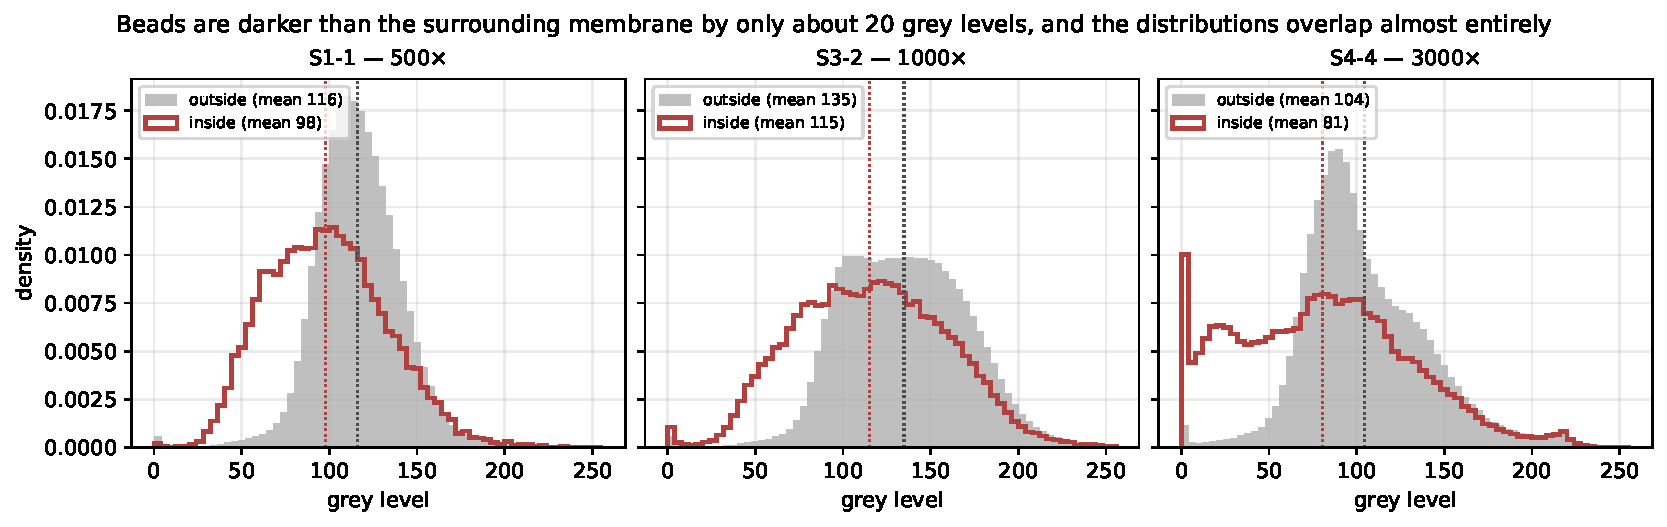
\includegraphics[width=\textwidth]{figures/fig_contrast.pdf}
    \caption{Grey-level distributions inside and outside the annotated beads, for
    one micrograph at each magnification. The means differ by about 20 levels
    while the distributions overlap almost entirely.}
    \label{fig:contrast}
\end{figure}

The parameters were tuned by grid search on the training partition of each fold
over morphological kernel size, minimum accepted object area in $\mu$m$^2$ and
marker suppression distance. The grid brackets the median annotated bead area of
about 38\,$\mu$m$^2$ from well below to well above, and the selected optimum falls
in the interior of the grid for all four folds, so the result is not an artefact
of too narrow a search. Its Segmentation Quality of 0.489 against a Recognition
Quality of 0.021 completes the picture: on the rare occasion it matches a bead the
mask is not unreasonable, but it almost never matches one.

\subsection{Method Comparison}
\label{sec:comparison}

% Generated by code/make_tables.py from results/metrics.json.
% Do not edit by hand: re-run the pipeline instead.
\begin{table}[htbp]
    \centering
    \caption{The mask-predicting methods under an identical protocol, averaged over
    the four leave-one-specimen-out folds. Counting error is the mean absolute
    percentage difference between the predicted and the annotated particle count.
    Detection-only methods are compared in Table~\ref{tab:counting}.}
    \label{tab:method_comparison}
    \begin{tabular}{lrrrr}
        \toprule
        Method & $\mathrm{AP}_{50}$ & AJI & Counting error (\%) & Merge rate (\%) \\
        \midrule
        Otsu + watershed & 0.001 & 0.067 & 580.4 & 17.4 \\
        U-Net + CC       & 0.152 & 0.305 & 44.2 & 48.7 \\
        Mask R-CNN       & 0.306 & 0.320 & 41.1 & 30.0 \\
        YOLOv8           & 0.254 & 0.254 & 93.2 & 34.5 \\
        \bottomrule
    \end{tabular}
\end{table}


Among the mask-predicting methods, Mask R-CNN leads on every metric measured and
the classical pipeline is last on all of them, so the fourth objective of
Section~\ref{sec:objectives} is met. The qualification concerns the two box-only
methods, absent from the mask-level columns. On counting, the only endpoint
defined identically for all six, Faster R-CNN is 1.7 points ahead of Mask R-CNN
(Section~\ref{sec:mask_branch}) while YOLOv5u is ahead of both on three folds and
far behind on the fourth (Section~\ref{sec:yolov5_results}). The ordering in
between depends on which metric is asked for, and that dependence is a result
rather than an inconvenience: YOLOv8 beats the U-Net on average precision, 0.254
against 0.152, and loses to it on counting, 99.3\% against 42.3\%.

The counting column separates the five failure modes more clearly than the
accuracy columns do. The classical pipeline fragments texture into objects,
over-counting by a factor of six. The U-Net fuses neighbours, under-counting by
42\% with an error entirely one-signed. YOLOv8 detects freely and fragments what
it detects, over-counting by 99\% with the highest recall and the highest split
rate, 28.5\%. YOLOv5u is the most accurate counter on three folds and the second
worst of the six on the fourth, its failure a loss of score calibration on one
specimen rather than a bias in one direction. Mask R-CNN errs in both directions:
its mean absolute counting error of 41.2\% is the lowest of the four
mask-predicting methods, while its mean signed error is $+3.0\%$, so most of its
absolute error cancels between micrographs that over- and under-count. That last
distinction matters for the application and is discussed in
Section~\ref{sec:counting}, since a method whose errors partly cancel is useful
for a population estimate in a way a biased method is not, while still being
unreliable for any single micrograph.

Table~\ref{tab:counting} restates the comparison on counting alone, the only
quantity defined identically for a method predicting masks and one predicting
only boxes. Where a row is marked \emph{box}, its average precision is computed on
bounding boxes rather than masks, and the two are not interchangeable.

% Generated by code/make_tables.py from results/metrics.json.
% Do not edit by hand: re-run the pipeline instead.
\begin{table}[htbp]
    \centering
    \caption{Counting accuracy under the leave-one-specimen-out protocol. Counts
    are pooled over the 11 held-out micrographs, while both error columns are
    averaged over them. Positive is an under-count and negative an over-count,
    and the two differ by however much the errors cancel. Methods marked (box)
    predict no masks, so their average precision is computed on boxes.}
    \label{tab:counting}
    \begin{tabular}{lrrrrr}
        \toprule
        Method & Detected & Annotated & Signed (\%) & Absolute (\%) & $\mathrm{AP}_{50}$ \\
        \midrule
        Otsu + watershed & 2205 & 606 & $-495.5$ & 502.1 & 0.001 (mask) \\
        U-Net + CC       & 325 & 606 & $+42.3$ & 42.3 & 0.152 (mask) \\
        Mask R-CNN       & 562 & 606 & $+3.0$ & 41.2 & 0.298 (mask) \\
        Faster R-CNN     & 602 & 606 & $-6.9$ & 39.5 & 0.305 (box) \\
        YOLOv8           & 1223 & 606 & $-90.2$ & 99.3 & 0.254 (mask) \\
        YOLOv5u          & 991 & 606 & $-63.0$ & 67.9 & 0.315 (box) \\
        \bottomrule
    \end{tabular}
\end{table}


Table~\ref{tab:ap_bands} decomposes average precision by object size. This matters
more here than the pooled figure suggests, since 82.8\% of the annotated particles
fall in the small band of COCO and 1.2\% in its large band
(Section~\ref{sec:small_objects}), so the pooled AP is close to an average over
a single band while appearing to describe three. $\mathrm{AP}_S$ is the column that
characterises this dataset, and it is the column that should be compared against the
small-object literature of Table~\ref{tab:coco_size} rather than against the pooled
COCO figures usually quoted.

% Generated by code/make_tables.py from results/metrics.json.
% Do not edit by hand: re-run the pipeline instead.
\begin{table}[htbp]
    \centering
    \caption{Average precision decomposed by object size, under the
    leave-one-specimen-out protocol. The bands are COCO's: small is below
    $32 \times 32$ pixels, large above $96 \times 96$. Since 82.8\% of the
    annotated particles are small and 1.2\% are large, $\mathrm{AP}_S$ is the
    column that describes this dataset; a dash marks a band the held-out ground
    truth does not populate, which cannot be scored.}
    \label{tab:ap_bands}
    \begin{tabular}{lrrrrrr}
        \toprule
        Method & AP & $\mathrm{AP}_{50}$ & $\mathrm{AP}_{75}$ &
        $\mathrm{AP}_S$ & $\mathrm{AP}_M$ & $\mathrm{AP}_L$ \\
        \midrule
        Otsu + watershed & 0.000 & 0.001 & 0.000 & --- & --- & --- \\
        U-Net + CC       & 0.049 & 0.152 & 0.031 & --- & --- & --- \\
        Mask R-CNN       & 0.113 & 0.282 & 0.069 & --- & --- & --- \\
        \bottomrule
    \end{tabular}
\end{table}


Two features of that table are worth stating. Four of the five learned methods
score higher on the medium band than on the small one, the expected direction and
the same effect Section~\ref{sec:magnification} measures against magnification;
the exception is YOLOv5u, at 0.126 against 0.132, a reversal of 0.006 belonging to
the method with the highest $\mathrm{AP}_S$ in the table. The large-band column
rests on the thinnest evidence in the chapter, since 1.2\% of the annotations are
large, fold Z4 contains none, and the column is averaged over three folds rather
than four. Nothing in this work should be concluded from it.

\subsection{Effect of Input Preprocessing}
\label{sec:preprocessing_results}

The four preprocessing variants of Section~\ref{sec:preprocessing_method} can be
characterised before any model is trained, by measuring on the annotations what
contrast each leaves available. Table~\ref{tab:contrast} reports the mean
grey-level separation between particle and mat and that separation divided by the
standard deviation of the background. The second is the one that matters, since a
transform that widens the gap while widening the spread by more has not made the
particles easier to find.

\begin{table}[htbp]
    \centering
    \caption{Particle-to-mat contrast under each preprocessing variant, measured
    over the 606 annotated particles before any training. $\Delta$ is the mean grey
    level outside a particle minus the mean inside and $\sigma$ is the background
    standard deviation.}
    \label{tab:contrast}
    \begin{tabular}{lrrrr}
        \toprule
        Preprocessing & $\Delta$ (grey levels) & $\sigma$ & $\Delta/\sigma$ &
        Change \\
        \midrule
        None (baseline)        & 18.0 & 33.2 & 0.550 & ---      \\
        Median filter, $3\times3$ & 18.3 & 30.5 & 0.612 & $+11\%$ \\
        Background subtraction & 20.3 & 34.9 & 0.593 & $+8\%$  \\
        CLAHE                  & 23.1 & 62.5 & 0.372 & $-32\%$ \\
        \bottomrule
    \end{tabular}
\end{table}

CLAHE is the instructive case. It produces the widest raw separation of the four, at
23.1 grey levels against 18.0 for the baseline, and on that number alone would be
the obvious choice. It also nearly doubles the background standard deviation, from
33.2 to 62.5, because the transform cannot distinguish a particle from the fibre
texture surrounding it and amplifies both. The usable contrast therefore falls by
almost a third. Figure~\ref{fig:preprocessing} shows this directly, as in the CLAHE
panel the fibres are as strongly modulated as the particle.

The other two transforms produce modest gains. The median filter improves
$\Delta/\sigma$ by 11\% by reducing the background spread rather than by increasing
the separation, which is the expected behaviour of a denoising filter on a signal
that it does not otherwise disturb. Background subtraction improves it by 8\%, and
its raw separation rises to 20.3, indicating that some of the measured
particle-to-mat difference in the untransformed images is attributable to
illumination gradient rather than to the particles.

\begin{figure}[htbp]
    \centering
    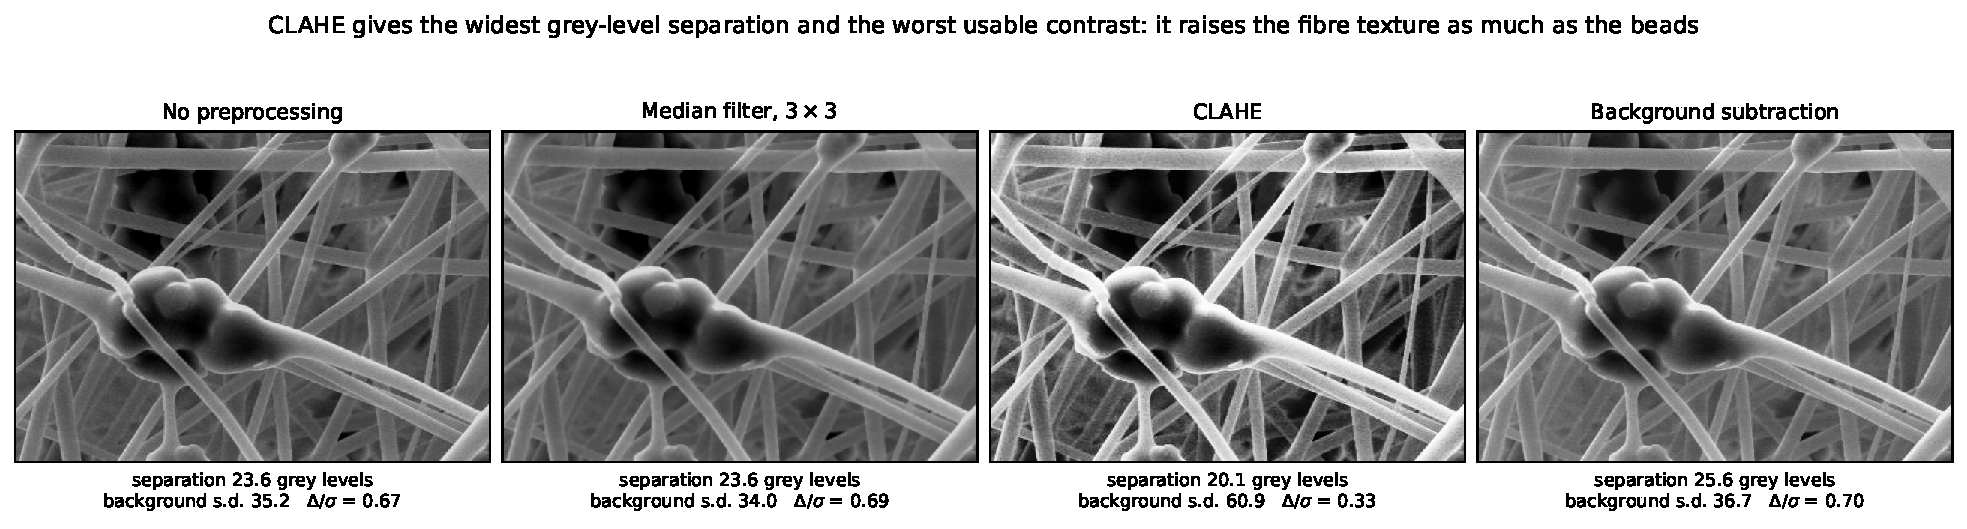
\includegraphics[width=\textwidth]{figures/fig_preprocessing.pdf}
    \caption{One region of Z6-4 under each preprocessing variant, with the
    contrast each yields over the whole dataset. In the CLAHE panel the particle is
    more strongly contrasted than in the baseline, and so is every fibre around
    it.}
    \label{fig:preprocessing}
\end{figure}

Two cautions attach to Table~\ref{tab:contrast}. It measures contrast, not
accuracy, and a convolutional detector is not a threshold, since it exploits
texture and shape this statistic ignores. And the models are initialised from
weights trained on natural images, so a transform moving the intensity statistics
far from that distribution may cost more than the contrast it buys.

% make_tables.py emits table_preprocessing.tex only when at least two variants
% have been evaluated, so this file compiles either way.
\IfFileExists{results/table_preprocessing.tex}{%
    % Generated by code/make_tables.py from results/metrics.json.
% Do not edit by hand: re-run the pipeline instead.
\begin{table}[htbp]
    \centering
    \caption{Effect of input preprocessing on Mask R-CNN, under the
    leave-one-specimen-out protocol. Architecture, schedule, folds and
    threshold-selection rule are identical across rows, so a difference is
    attributable to the input transform alone. The second column is the
    particle-to-mat contrast measured directly on the annotations before any
    training: the mean grey-level separation divided by the standard deviation of
    the background, which is the contrast a filter actually has to work with.}
    \label{tab:preprocessing}
    \begin{tabular}{lrrrrr}
        \toprule
        Preprocessing & Contrast & $\mathrm{AP}_{50}$ & $\mathrm{AP}_S$ &
        AJI & Counting error (\%) \\
        \midrule
        None (baseline)            &  0.55 & 0.306 & 0.116 & 0.320 & 41.1 \\
        Median filter, 3x3         &  0.61 & 0.289 & 0.108 & 0.320 & 36.4 \\
        CLAHE                      &  0.37 & 0.262 & 0.094 & 0.290 & 39.3 \\
        Background subtraction     &  0.59 & 0.263 & 0.104 & 0.307 & 31.3 \\
        \bottomrule
    \end{tabular}
\end{table}
%
}{}

\textbf{No transform improves detection over the untransformed input.} Mask R-CNN
scores $\mathrm{AP}_{50} = 0.298$ on the raw micrographs, against 0.289 with the
median filter, 0.263 with background subtraction and 0.262 with CLAHE, and the
ordering on $\mathrm{AP}_S$ is the same; architecture, schedule, folds and
threshold-selection rule were identical across the four rows. The contrast
statistic therefore succeeded at one of its two jobs: it identified the harmful
transform correctly, since CLAHE loses a third of the usable contrast and is last
or joint-last on every accuracy column, but failed to identify a beneficial one,
having predicted gains of 11\% and 8\% for the median filter and background
subtraction, both of which cost detection accuracy instead. The two cautions
recorded above, before the runs rather than after them, are the likeliest
explanation.

One row points the other way, and it is the row the laboratory cares about most.
Background subtraction gives the lowest counting error of the four variants,
31.5\% against 41.2\%, while losing 0.035 of $\mathrm{AP}_{50}$, and it has the
lowest split rate of any Mask R-CNN variant, 11.6\% against 13.8\%. What separates
the two on counting is not the average instance behaviour but the tails: the two
worst frames of the baseline over-count by 119\% and 83\%, and background
subtraction brings them to 27\% and 21\%, at the cost of turning a near-miss on
the densest micrograph into a 50\% under-count. The reading this supports is
narrow. Removing the illumination gradient does not help the detector find beads
and on this evidence slightly hinders it; what it does is suppress the runaway
over-counts on sparsely populated frames, which is what a mean of per-micrograph
percentage errors rewards most. These runs cannot say which difference would
survive a second seed (Section~\ref{sec:reliability}).

\subsection{Effect of Threefold Magnification}
\label{sec:upsample_results}

Section~\ref{sec:magnification} finds that the model detects best where the beads
occupy the most pixels. That finding suggests an intervention that costs nothing in
acquisition, namely resampling the dataset itself. Each micrograph and its
annotation are magnified threefold with bicubic interpolation, the network is
trained and run at the magnified scale, and its predictions are mapped back to
native resolution before scoring, so both configurations are measured against
the same ground truth in the same coordinate frame.

% Emitted only when the magnified run has been evaluated.
\IfFileExists{results/table_upsample.tex}{%
    % Generated by code/make_tables.py from results/metrics.json.
% Do not edit by hand: re-run the pipeline instead.
\begin{table}[htbp]
    \centering
    \caption{Effect of magnifying the dataset threefold by bicubic
    interpolation, under the leave-one-specimen-out protocol. Image and
    annotation are resampled together and the predictions are mapped back to
    native resolution before scoring, so both rows are measured against the same
    ground truth. Architecture, schedule, folds and threshold-selection rule are
    identical.}
    \label{tab:upsample}
    \begin{tabular}{lrrrr}
        \toprule
        Input scale & $\mathrm{AP}_{50}$ & $\mathrm{AP}_S$ & AJI &
        Counting error (\%) \\
        \midrule
        Native resolution            & 0.298 $\pm$ 0.059 & 0.116 & 0.325 $\pm$ 0.053 & 41.1 \\
        $3\times$ bicubic            & 0.373 $\pm$ 0.039 & 0.158 & 0.359 $\pm$ 0.052 & 42.7 \\
        \bottomrule
    \end{tabular}
\end{table}
%
}{}

The effect is the largest of any input-side intervention reported here.
$\mathrm{AP}_{50}$ rises from 0.298 to 0.373 and $\mathrm{AP}_S$ from 0.116 to
0.158, gains of 0.075 and 0.042 against a between-fold standard deviation of 0.059
and 0.035 respectively. AJI rises from 0.325 to 0.359 and Panoptic Quality from
0.351 to 0.394, and the decomposition says where the gain comes from: Recognition
Quality rises from 0.486 to 0.541 while Segmentation Quality moves only from 0.719
to 0.733. Pooled over the 11 held-out micrographs the model now matches 397 of the
606 annotated beads against 271 before, a recall of 0.655 against 0.447, at an
essentially unchanged precision of 0.493 against 0.482.

Interpolation adds no information, and the result should not be read as though it
did. What changes is the number of pixels per object: the median bead at
$500\times$ goes from 14 pixels across to 42, moving it from the size at which the
finest pyramid level and the smallest anchor are both marginal to one at which
neither is. The gain is therefore evidence for the diagnosis of
Section~\ref{sec:magnification}, obtained by changing only the scale of the input.

The counting endpoint does not follow. Mean absolute counting error is 44.0\%
against 41.2\%, and the aggregate turns from a deficit into a surplus, 806 objects
against 606 annotated where the baseline reported 562. Finding more beads has
meant fragmenting more of them, the split rate rising from 13.8\% to 18.0\% and
the merge rate from 24.9\% to 28.9\%, which is the same trade the instance methods
make against each other in Section~\ref{sec:comparison}, reappearing within one
architecture.

The cost is not negligible. Training takes 26.3 minutes per fold against 10.3, and
inference has to be tiled, since a magnified micrograph is $3072 \times 2208$ and
the mask head allocates one full-resolution mask per detection. For a laboratory
whose endpoint is the size distribution the gain is worth two and a half times the
training time; for one whose endpoint is the count, this run offers nothing.

\subsection{Qualitative Examples}

\begin{figure}[htbp]
    \centering
    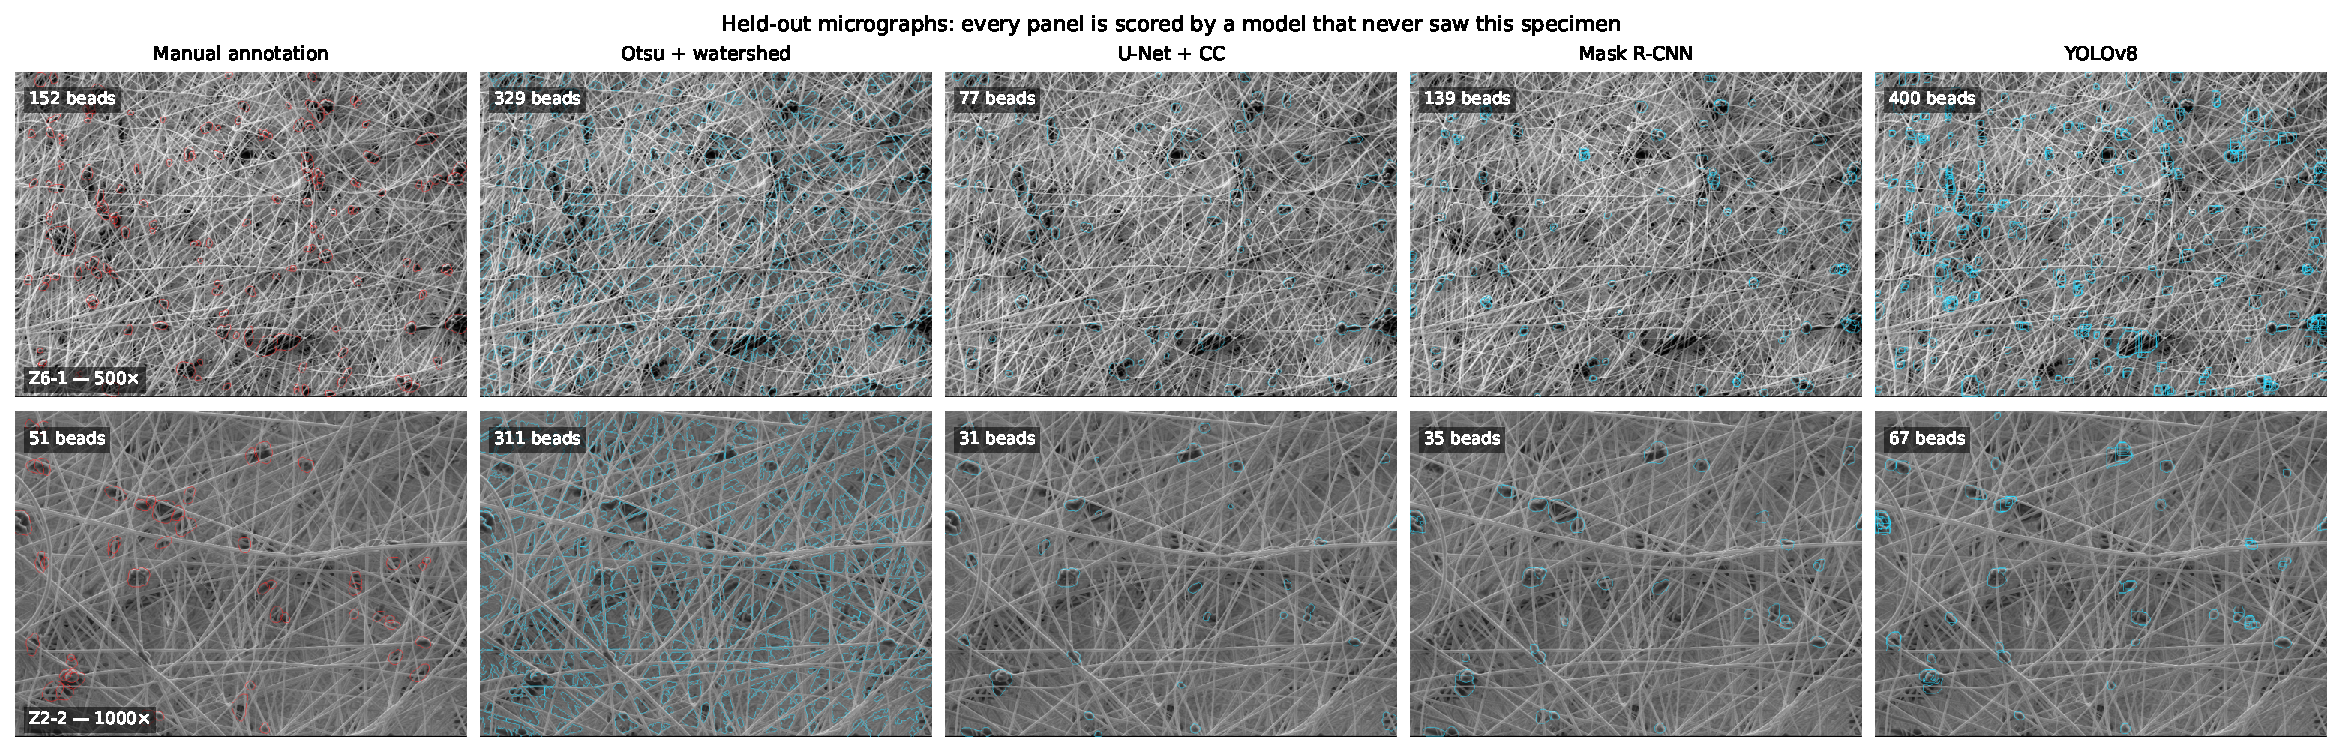
\includegraphics[width=\textwidth]{figures/fig_qualitative.pdf}
    \caption{The four mask-predicting methods on two held-out micrographs, Z6-1
    at $500\times$ and Z2-2 at $1000\times$, each from a model that never saw that
    specimen. Red outlines are the manual annotation, blue the prediction. Faster
    R-CNN predicts no masks and is absent.}
    \label{fig:qualitative}
\end{figure}

Figure~\ref{fig:qualitative} shows the mask-predicting methods on two held-out
micrographs, and each numerical finding above has a visible counterpart in it.

On Z6-1 the annotator marked 152 beads. The classical pipeline returns 329 regions
that tile the frame more or less irrespective of where the beads are, which is the
visual form of an $\mathrm{AP}_{50}$ of 0.001. The U-Net returns 77 regions, half
the true count, visibly larger than individual beads because adjacent beads have
been absorbed into single components: the 48.7\% merge rate made visible. YOLOv8
returns 400, hitting the detection cap, with many small outlines subdividing
single annotated beads. Mask R-CNN returns 139 regions that correspond
recognisably to individual beads, and its errors are of a different kind, beads
missed entirely rather than fused or fragmented. On Z2-2, where the annotator
marked 51 beads, the same pattern holds at a different scale: the classical
pipeline returns 311 regions, the U-Net 31 and Mask R-CNN 35, both under-counting
although the U-Net's regions again span neighbouring beads, while YOLOv8 returns
67.

\section{The Cost of a Naive Split}
\label{sec:leakage}

% Generated by code/make_tables.py from results/metrics.json.
% Do not edit by hand: re-run the pipeline instead.
\begin{table}[htbp]
    \centering
    \caption{The same model under a specimen-wise protocol and under a random
    split over the 11 images, with identical fold sizes.}
    \label{tab:leakage}
    \begin{tabular}{lrrr}
        \toprule
        Protocol & $\mathrm{AP}_{50}$ & AJI & Counting error (\%) \\
        \midrule
        Random split over images & 0.303 & 0.313 & 43.9 \\
        Leave-one-specimen-out   & 0.298 & 0.325 & 41.2 \\
        \midrule
        Difference & 0.005 & -0.012 & 2.7 \\
        \bottomrule
    \end{tabular}
\end{table}


This is a negative result and it is reported as measured.

Evaluating the same model under a random split over the 11 micrographs, with fold
sizes identical to the specimen-wise protocol, gives
$\mathrm{AP}_{50} = 0.303$ against 0.298 for leave-one-specimen-out, a difference
of 0.005 in favour of the random split, against a between-fold standard deviation
of 0.059. The other two metrics run the other way, as AJI is 0.313 against 0.325
and mean absolute counting error 43.9\% against 41.2\%. Only one of the three
differences points in the direction a leak would produce, and it is a twelfth of
the between-fold spread. On this dataset the naive protocol does not measurably
overstate performance.

The second objective of Section~\ref{sec:objectives} asked for a demonstration
that the naive alternative overstates performance, and that demonstration did not
materialise. The protocol remains the correct one, but on the strength of
structural argument rather than of measured inflation. Three factors plausibly
explain the absence of a gap, and the first is the most likely.

\textbf{The leak that mattered had already been removed.} The 132 pre-computed
augmented copies were discarded before any partitioning
(Section~\ref{sec:supplied_aug}). They are near-duplicates of their originals, so
letting them cross a partition boundary would put a transformed version of a test
image directly into training. The remaining dependence between two micrographs of
one specimen at different magnifications is far weaker, being different fields of
view at different scales that share only the general morphology of the specimen.

\textbf{There is little headroom to inflate.} A protocol can only flatter a model
capable of memorising. At $\mathrm{AP}_{50} = 0.30$ and a Recognition Quality of
0.49, this model is under-fitting rather than memorising, and
Section~\ref{sec:generalisation} measures that directly.

\textbf{With 11 images, both protocols are noisy.} The folds of the random split
range from $\mathrm{AP}_{50} = 0.199$ to 0.423, a spread of 0.224, against 0.223
to 0.355 for the specimen-wise folds, a spread of 0.132. The random protocol gave
a mean higher by 0.005 and a fold-to-fold spread 1.7 times as wide, which is
reason to prefer the specimen-wise protocol independently of any bias argument: it
is the more stable estimator, and on four folds stability is worth more than it
would be on forty.

\section{Training Accuracy against Test Accuracy}
\label{sec:generalisation}

Section~\ref{sec:leakage} argues that there is little headroom for a protocol to
inflate, because the model is under-fitting rather than memorising. That argument
can be measured. The model of each fold is scored a second time on the eight
micrographs on which it was trained, by the same code and against the same
annotations.

% Emitted only when at least one method has recorded a training partition.
\IfFileExists{results/table_generalisation.tex}{%
    % Generated by code/make_tables.py from results/metrics.json.
% Do not edit by hand: re-run the pipeline instead.
\begin{table}[htbp]
    \centering
    \caption{Training accuracy against test accuracy under the
    leave-one-specimen-out protocol. Each fold's model is scored on the
    micrographs it was trained on and on the specimen it was held out from, by
    the same code and against the same annotations. The gap is train minus test
    in each metric's own units, so the model favours what it has already seen
    when the $\mathrm{AP}_{50}$ gap is positive and when the counting gap is
    negative. The training figure is not a result in
    its own right -- it is measured on data the optimiser was given -- but the
    distance between the two columns is: it separates a model that has memorised
    its training specimens from one that is limited by the difficulty of the
    task. No pooled figure is given because a micrograph belongs to the training
    partition of three of the four folds, so pooling would weight specimens by
    how often they recur.}
    \label{tab:generalisation}
    \begin{tabular}{lrrrrrr}
        \toprule
        & \multicolumn{3}{c}{$\mathrm{AP}_{50}$} &
        \multicolumn{3}{c}{Counting error (\%)} \\
        \cmidrule(lr){2-4} \cmidrule(lr){5-7}
        Method & Train & Test & Gap & Train & Test & Gap \\
        \midrule
        Mask R-CNN               & 0.437 & 0.298 & +0.139 & 32.6 & 41.1 & -8.5 \\
        Faster R-CNN             & 0.412 & 0.305 & +0.107 & 35.7 & 37.8 & -2.2 \\
        Mask R-CNN, $3\times$ bicubic & 0.459 & 0.373 & +0.086 & 46.0 & 42.7 & +3.3 \\
        \bottomrule
    \end{tabular}
\end{table}
%
}{}

The gap is real and modest. Mask R-CNN scores $\mathrm{AP}_{50} = 0.437$ on data
it has seen against 0.298 on data it has not. The ratio is the wrong way to read
it: what matters is that 0.437 is itself a modest score, so the model does not
come close to fitting even its training partition. A network that had memorised
eight micrographs would score near ceiling on them and this one does not, so the
deficit reported throughout the chapter is one of capacity and training budget
rather than of generalisation.

Two comparisons within the table sharpen that. Faster R-CNN, the same architecture
with the mask head removed, has a smaller gap than Mask R-CNN, 0.107 against
0.139, the expected direction for a model with fewer parameters to fit. The
threefold-magnified model has the smallest gap of the three, 0.086, together with
the highest test score, so its gain is not bought by fitting the training data
harder, which is what a resampling artefact would have looked like.

The counting column is reported for completeness. Mask R-CNN counts better on its
training partition than on its test specimen, 32.5\% against 41.2\%, Faster R-CNN
barely distinguishes the two, 35.7\% against 39.5\%, and the magnified model
counts \emph{worse} on training than on test, 45.6\% against 44.0\%. That
inversion is not a paradox, since the counting figure is an unweighted mean of
per-micrograph percentage errors dominated by the sparsely populated frames. The
training column is not a result in its own right, and it is optimistic twice over,
since the score threshold was itself chosen by maximising $F_1$ on that same
partition. No pooled training figure is given, because a micrograph belongs to the
training partition of three folds.

\section{Behaviour Across Magnification}
\label{sec:magnification}

% Generated by code/make_tables.py from results/metrics.json.
% Do not edit by hand: re-run the pipeline instead.
\begin{table}[htbp]
    \centering
    \caption{Mask R-CNN performance by magnification, pooled over the four
    leave-one-specimen-out folds. Every micrograph is scored by the model that
    did not see its specimen.}
    \label{tab:magnification}
    \begin{tabular}{lrrrrr}
        \toprule
        Magnification & Images & Beads & $\mathrm{AP}_{50}$ & AJI & $|$Counting error$|$ (\%) \\
        \midrule
        $500\times$ & 3 & 325 & 0.227 & 0.233 & 29.1 \\
        $1000\times$ & 4 & 229 & 0.342 & 0.316 & 48.8 \\
        $3000\times$ & 4 & 52 & 0.396 & 0.384 & 42.6 \\
        \bottomrule
    \end{tabular}
\end{table}


Detection improves monotonically with magnification, the opposite of what the
sample sizes alone would predict. The $3000\times$ group is the smallest in the
dataset, 52 beads across four micrographs against 325 at $500\times$, and is
nonetheless the group on which the model detects best, at
$\mathrm{AP}_{50} = 0.396$ and AJI 0.384 against 0.227 and 0.233 at $500\times$.

Object size and not sample size is therefore the binding constraint. The median
bead is 14 pixels across at $500\times$ and 76 at $3000\times$. At 14 pixels a
bead spans roughly the receptive field of the finest pyramid level and is only a
few pixels larger than the smallest anchor, so its boundary is decided by a
handful of pixels, whereas at 76 pixels it is comfortably resolved.
Table~\ref{tab:magnification} shows that the feature pyramid and the rescaled
anchors narrow the gap without closing it.

Counting does not follow the same ordering. The mean absolute counting error is
lowest at $500\times$, 29.1\%, and higher at both other settings, 48.8\% at
$1000\times$ and 42.6\% at $3000\times$. Part of that is an arithmetic property of
the field of view rather than a contradiction of the detection result, since a
$3000\times$ micrograph carries 13 annotated beads on average and as few as four,
so one spurious detection on a four-bead frame is a 25\% error while one on the
152-bead Z6-1 is 0.7\%. The ordering between $1000\times$ and $3000\times$ is not
evidence of anything: each group holds three or four micrographs and the mean of
each is dominated by one of them, the 48.8\% at $1000\times$ carried by Z6-2,
over-counted by 119\%, and the 29.1\% at $500\times$ by Z5-1, under-counted by
75\%, so removing either frame reverses the ranking. The detection columns, which
average over hundreds of objects, are the ones this table supports.

The practical consequence follows from the detection trend alone. High
magnification gives better boundaries and therefore a better size distribution. If
both quantities are wanted from one setting, $1000\times$ is the defensible
compromise, within 0.054 of the best $\mathrm{AP}_{50}$ while framing 229
annotated beads against the 52 available at $3000\times$. What these results
cannot support is a recommendation based on the counting column itself, and with
only 52 beads the $3000\times$ figures should be read as indicative.

\section{Physical Quantification}

\subsection{Bead Count and Areal Density}
\label{sec:counting}

Summed over all 11 held-out micrographs, Mask R-CNN reports 562 beads against 606
annotated, an aggregate under-count of $+7.3\%$. That figure is far more
favourable than the method deserves, since it is the sum of errors that largely
cancel. Per specimen the mean signed error runs from $+40.3\%$ on Z4, the largest
under-count, to $-64.7\%$ on Z6, the largest over-count, and per micrograph from
$+74.5\%$ on Z5-1 to $-119.4\%$ on Z6-2, while the mean absolute error is 41.2\%
against a mean signed error of $+3.0\%$. A single micrograph is therefore not a
reliable measurement, and 7.3\% against 41.2\% is a factor of six, none of which
comes from the model being right.

That cancellation is a property of the method rather than of aggregation. Faster
R-CNN aggregates to $+0.7\%$ against a mean absolute error of 39.5\%, a wider gap
still. YOLOv5u gains nothing, its aggregate of $-63.5\%$ nearly matching its mean
absolute error because its error is one-signed and concentrated on a single
specimen, while the aggregate of $-101.8\%$ for YOLOv8 is worse than its mean
absolute error of 99.3\%. A
laboratory pooling many micrographs would gain roughly a factor of six from Mask
R-CNN, more from Faster R-CNN, and nothing from either YOLO model. That
distinction appears in no accuracy column in this chapter.

Figure~\ref{fig:counting} plots the two counts against each other. Four of the
eleven micrographs fall within 25\% of the annotated count, and the largest errors
lie on both sides: Z5-1, the second most densely populated micrograph, is
under-counted by three quarters, while Z6-2 is over-counted by 119\% and Z6-4 by
83\%. The extremes are at both ends of the density range, which is where a merge
on the dense frames, or a spurious split on the sparse ones, costs most.

\begin{figure}[htbp]
    \centering
    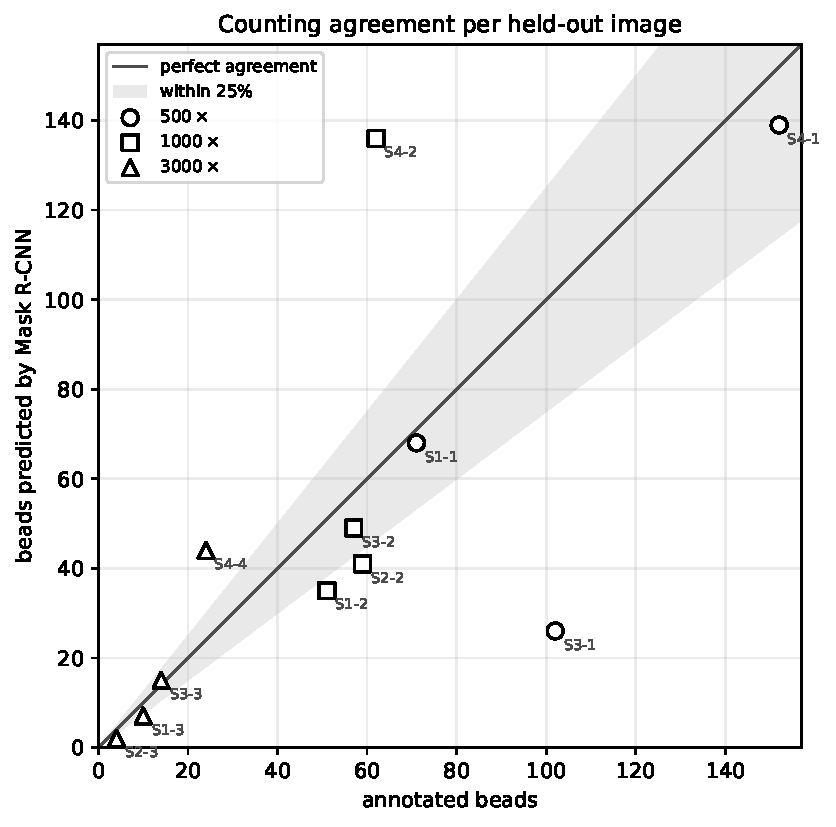
\includegraphics[width=0.78\textwidth]{figures/fig_counting.pdf}
    \caption{Predicted against annotated bead count for each held-out micrograph,
    with marker shape indicating magnification. Points on the diagonal agree
    exactly.}
    \label{fig:counting}
\end{figure}

Areal density inherits this behaviour directly, since it is the count divided by a
known physical area. On Z2-1 the model reports 292 beads\,mm$^{-2}$ against 305
measured manually, on Z5-1 it reports 112 against 438, and on Z6-2, 2338 against
1066. The fifth objective of Section~\ref{sec:objectives} is met in the sense that
these quantities are reported and compared, but the comparison does not support
using the pipeline as a drop-in replacement for manual counting on a single field.

\subsection{Size Distribution Agreement}

% Generated by code/make_tables.py from results/metrics.json.
% Do not edit by hand: re-run the pipeline instead.
\begin{table}[htbp]
    \centering
    \caption{Predicted bead size distribution against the manual ground truth,
    pooled over the 11 held-out micrographs. Diameters are equivalent circular
    diameters in micrometres.}
    \label{tab:physical}
    \begin{tabular}{lrrrrr}
        \toprule
        Source & Beads & Median $d$ ($\mu$m) & IQR ($\mu$m) & KS $D$ & $p$ \\
        \midrule
        Manual annotation & 606 & 7.97 & [6.42, 10.16] & --- & --- \\
        \midrule
        Otsu + watershed & 2205 & 8.58 & [6.72, 10.99] & 0.105 & 4.9e-05 \\
        U-Net + CC       & 325 & 8.78 & [6.48, 12.09] & 0.154 & 7.5e-05 \\
        Mask R-CNN       & 562 & 7.72 & [5.65, 9.14] & 0.139 & 2.4e-05 \\
        YOLOv8           & 1223 & 7.81 & [6.05, 10.39] & 0.075 & 2.0e-02 \\
        \bottomrule
    \end{tabular}
\end{table}


The predicted median diameter of Mask R-CNN is 7.72\,$\mu$m against 7.97\,$\mu$m
measured manually, a difference of 3.2\%, with an interquartile range of 5.65 to
9.14\,$\mu$m against 6.42 to 10.16\,$\mu$m. The predicted distribution is narrower
and smaller, consistent with a detector that misses the beads hardest to delineate
and trims the boundaries of those it keeps.

All four two-sample Kolmogorov--Smirnov tests reject the hypothesis that the
predicted and manual distributions are the same, three at $p < 10^{-3}$ and that
of YOLOv8 at $p = 0.02$. That should not be over-read, since with hundreds of
samples on each side the test is sensitive to differences far smaller than those
that matter for process optimisation, and a 3.2\% error in median bead diameter is
smaller than the 15\% spread the same annotation shows across magnifications.
Figure~\ref{fig:size_agreement} shows that Mask R-CNN tracks the manual
distribution closely through its bulk and falls short in the tail above roughly
15\,$\mu$m.

\begin{figure}[htbp]
    \centering
    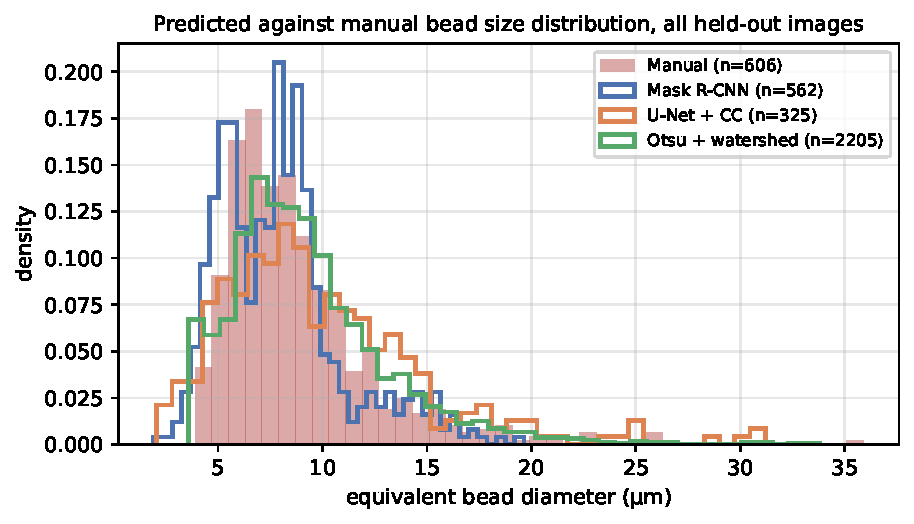
\includegraphics[width=0.9\textwidth]{figures/fig_size_agreement.pdf}
    \caption{Predicted against manual bead size distributions, pooled over all
    11 held-out micrographs.}
    \label{fig:size_agreement}
\end{figure}

Two rows of Table~\ref{tab:physical} are a warning rather than a finding. Of the
four methods, YOLOv8 has the \emph{lowest} KS statistic at $D = 0.075$ and the
classical pipeline the second lowest at $D = 0.105$, and these are the two that
over-count by 99\% and 495\%. Both achieve their agreement by reporting far more
objects than exist, whose sizes happen to span a similar range to the real beads,
while Mask R-CNN, the best method by every other measure here, has a worse $D$ than
both.

Distributional agreement alone is therefore not a sufficient criterion, since a
method can reproduce the size distribution of a population that it has substantially
failed to identify. Had this work reported only the size distribution, which is one
of the two quantities that the laboratory asked for, it would have ranked the two
worst methods first.

\section{Discussion}

\subsection{Key Findings}

\textbf{Instance segmentation is the right formulation, and the reason is
separation rather than accuracy.} Mask R-CNN and the U-Net differ by 0.020 in AJI
but by 0.157 in Panoptic Quality and by 23.8 percentage points in merge rate, and
the annotation itself contains 8.8\% overlapping bead pixels. The formulation
trades one error for another rather than eliminating error: the U-Net merges
48.7\% of beads and splits none, Mask R-CNN merges 24.9\% and splits 13.8\%, and
YOLOv8 merges 34.5\% and splits 28.5\%.

\textbf{Counting can be far more accurate than the mean figures suggest, and the
obstacle is score calibration rather than detection.} YOLOv5u counts three of the
four held-out specimens to within 8.2\%, 15.0\% and 18.3\% and misses the fourth
by 212.5\%, mostly because the training partition set a threshold of 0.10 on that
fold against 0.20 to 0.35 on the others.

\textbf{Small objects, not scarce labels, are the binding constraint on
detection.} Detection is best where the data are scarcest and the objects largest,
and magnifying the dataset threefold raises $\mathrm{AP}_{50}$ from 0.298 to 0.373
and recall from 0.447 to 0.655 without adding information, which is precisely why
it is evidence. The model under-fits rather than memorises, reaching 0.437 on the
micrographs it trained on, so the shortfall is one of capacity and training budget.

\textbf{The absolute performance is not yet sufficient for unattended use.} An
$\mathrm{AP}_{50}$ of 0.298 and a per-micrograph counting error of 41.2\% do not support
replacing a human operator on a single micrograph, although the aggregate error
over eleven micrographs is 7.3\%. Classical thresholding is not viable at all, at
$\mathrm{AP}_{50} = 0.001$, for a reason measurable in the micrographs: about 20
grey levels separate a bead from the surrounding mat.

\textbf{Preprocessing did not improve detection, and one variant improved
counting.} No transform beat the raw input on $\mathrm{AP}_{50}$, while background
subtraction cut counting error from 41.2\% to 31.5\%. And the specimen-wise
protocol did not change the headline number, but reduced the fold-to-fold spread
by a third, which is a weaker claim than the one anticipated in
Section~\ref{sec:objectives} and the one the data support.

\subsection{Comparison with the Literature}

A direct numerical comparison with published work is not possible, since no public
benchmark for beads in electrospun mats exists and the AP values reported
here are specific to this annotation and protocol. Three qualitative comparisons
can be made.

The merge behaviour of semantic segmentation with connected-component
post-processing is well documented in the nuclei segmentation literature, and
motivates the shape-prior methods of Schmidt et al.\ \cite{schmidt2018stardist}
and Stringer et al.\ \cite{stringer2021cellpose} and the weighted-boundary loss of
the original U-Net \cite{ronneberger2015unet, falk2019unet}. The 48.7\% merge rate
measured here is a direct instance of that effect.

The difficulty of small objects for region-based detectors is likewise a known
property of the architecture, and is what the feature pyramid
\cite{lin2017feature} was introduced to address. The one-stage weakness on small
objects reported for the YOLO family \cite{redmon2016yolo, lin2020focal} appears
in one of the two models tested and not the other: YOLOv8 reaches an
$\mathrm{AP}_S$ of 0.091 against 0.116 for Mask R-CNN, while YOLOv5u reaches
0.132, the highest of the six. At this object size the weakness is therefore not a
property of the family as such, and four folds cannot establish whether the
backbone or the mask branch accounts for the gap.

The absolute values are well below those reported on nuclei benchmarks such as the
dataset of Kumar et al.\ \cite{kumar2017dataset}, and the relevant difference is
training set size: those results rest on tens of thousands of annotated objects
against 606 here from four specimens.

\subsection{Limitations}
\label{sec:limitations}

The limitations below follow from the dataset and from the experimental design.

\textbf{Four specimens.} The strongest claim this dataset can support is
generalisation across four specimens of what appears to be one material system. It
cannot establish generalisation to a different polymer, solvent or instrument.

\textbf{Fifty-two beads at $3000\times$.} The highest magnification is represented
by only 52 annotated objects, so the per-magnification result for $3000\times$,
which is also the most striking finding of Section~\ref{sec:magnification}, rests
on a small sample and should be read as indicative.

\textbf{One annotator.} All 606 annotations come from a single source, so
annotator bias cannot be distinguished from ground truth and no inter-annotator
agreement can be reported. At $\mathrm{AP}_{50} = 0.298$ it is not known how much
of the shortfall is model error and how much is disagreement that a second
annotator would also show.

\textbf{Single class.} The annotation does not distinguish beads from locally
thickened fibre segments, so the boundary between the two rests on the implicit
judgement of the annotator. Several of the false positives on visual inspection
are objects of this ambiguous kind.

\textbf{No hyperparameter search.} Every model was trained once, with the
configuration of Table~\ref{tab:training_config}, for 1500 iterations. The
reported figures are what that configuration produces and not the best achievable.

\textbf{Neither YOLO model was given a matched input budget.} Both were trained on
whole $1024$-pixel micrographs where the region-based models saw
$512 \times 512$ crops, because their data pipeline expects a fixed image
directory. Their accuracy figures are therefore not a like-for-like architectural
comparison, and their threefold training cost is largely a consequence of that
difference.

\textbf{The detection cap binds for YOLOv8 on one micrograph.} It returns exactly
400 objects on Z6-1, so its over-count there, and hence its pooled counting error,
is a lower bound rather than a measurement. It does not bind for any other method,
the largest output of YOLOv5u on the same micrograph being 292.

\textbf{The YOLOv5u counting figure averages two different behaviours.} Its mean
of 67.9\% describes neither, since three folds fall between 8.2\% and 18.3\% and
the fourth at 212.5\%. The threshold diagnostic of
Section~\ref{sec:yolov5_results} is labelled a diagnostic for the same reason, as
it re-scores held-out predictions.

\subsection{Reliability of the Reported Numbers}
\label{sec:reliability}

Each configuration was run \emph{once}, with a fixed seed of 0. No seed was varied
and no configuration was repeated, so every figure in this chapter is a single-run
point estimate and none of the reported standard deviations measures run-to-run
variability. They are between-fold spreads over four folds, which is a different
and weaker quantity: they describe how much the result depends on which specimen
was held out. Counting error is the exception, summarised over the eleven
micrographs rather than the four folds; a between-fold spread of it is named as
such where one is quoted.

With four folds, a standard deviation is itself estimated from four numbers and is
not a confidence interval. Varoquaux \cite{varoquaux2018crossvalidation} shows
that cross-validated estimates from small samples carry error bars far wider than
is usually assumed, and that differences well below them are routinely reported as
findings. Two comparisons here are the most exposed. The protocol comparison of
Section~\ref{sec:leakage} turns on 0.005 in $\mathrm{AP}_{50}$, about a twelfth of
the between-fold spread, so the correct reading is that no difference was detected
rather than that the protocols were shown equivalent. The preprocessing comparison
turns on differences of 0.009 to 0.036 against a spread of 0.059, where the
direction is consistent across the three variants but no single pairwise
difference is resolved.

The magnification ablation of Section~\ref{sec:upsample_results} is the one
input-side comparison not in that position. Its gain of 0.075 in
$\mathrm{AP}_{50}$ exceeds the between-fold standard deviation of the baseline and
holds on three folds, by 0.059, 0.181 and 0.096 on Z2, Z5 and Z6. The exception is
Z4, where the magnified model scores 0.317 against 0.355, this being the fold of
63 beads across two micrographs. These runs resolve that difference in the sense
that its size exceeds the noise, but cannot put an interval on it.

What can be stated robustly is the ranking of the classical pipeline against the
learned methods, consistent across every metric and every fold; the direction and
magnitude of the merge, split and counting biases, which are large and
systematically signed; and the factor of six between per-micrograph and aggregate
counting error. What cannot is any small difference between two similar numbers,
including the ordering of Mask R-CNN against YOLOv8 on average precision and that
of YOLOv5u against Faster R-CNN, where 0.315 against 0.305 is set against
between-fold spreads of 0.049 and 0.073.

\section{Summary}

Mask R-CNN leads the mask-predicting alternatives on every metric, at
$\mathrm{AP}_{50} = 0.298 \pm 0.059$, AJI $0.325 \pm 0.053$ and a counting error
of 41.2\%, and reaches neither criterion of Section~\ref{sec:objectives}. The
comparison locates what the instance formulation contributes, the separation of
touching objects rather than mask accuracy, and what it does not: the mask branch
is worth every mask-level measurement and nothing on the count, while the two
box-only methods clear the 0.30 criterion on the quantity it was originally
measured on. YOLOv5u counts three specimens better than anything else here and the
fourth far worse, for a reason that is score calibration rather than detection.

On the input side, object size in pixels is the binding constraint: detection
improves with magnification although the highest magnification holds the fewest
beads, and resampling the dataset threefold reproduces the gain without adding
information. No preprocessing variant improved detection, one improved counting,
and the naive partitioning protocol did not measurably overstate performance.
Predicted bead diameters agree with the manual measurement to 3.2\% in the median,
while counting remains too variable per micrograph, 41.2\% against an aggregate
7.3\% over eleven, for unattended use.
